%%
%% This is file `sample-sigconf-authordraft.tex',
%% generated with the docstrip utility.
%%
%% The original source files were:
%%
%% samples.dtx  (with options: `all,proceedings,bibtex,authordraft')
%% 
%% IMPORTANT NOTICE:
%% 
%% For the copyright see the source file.
%% 
%% Any modified versions of this file must be renamed
%% with new filenames distinct from sample-sigconf-authordraft.tex.
%% 
%% For distribution of the original source see the terms
%% for copying and modification in the file samples.dtx.
%% 
%% This generated file may be distributed as long as the
%% original source files, as listed above, are part of the
%% same distribution. (The sources need not necessarily be
%% in the same archive or directory.)
%%
%%
%% Commands for TeXCount
%TC:macro \cite [option:text,text]
%TC:macro \citep [option:text,text]
%TC:macro \citet [option:text,text]
%TC:envir table 0 1
%TC:envir table* 0 1
%TC:envir tabular [ignore] word
%TC:envir displaymath 0 word
%TC:envir math 0 word
%TC:envir comment 0 0
%%
%% The first command in your LaTeX source must be the \documentclass
%% command.
%%
%% For submission and review of your manuscript please change the
%% command to \documentclass[manuscript, screen, review]{acmart}.
%%
%% When submitting camera ready or to TAPS, please change the command
%% to \documentclass[sigconf]{acmart} or whichever template is required
%% for your publication.
%%
%%
% ISS 2026 / PACM HCI review format: single column, line-numbered, anonymous.
\documentclass[manuscript,review,anonymous]{acmart}
%%
%% \BibTeX command to typeset BibTeX logo in the docs
\AtBeginDocument{%
  \providecommand\BibTeX{{%
    Bib\TeX}}}

%% Rights management information.  This information is sent to you
%% when you complete the rights form.  These commands have SAMPLE
%% values in them; it is your responsibility as an author to replace
%% the commands and values with those provided to you when you
%% complete the rights form.






\setcopyright{none}
\copyrightyear{2026}
\acmYear{2026}


%%
%% Submission ID.
%% Use this when submitting an article to a sponsored event. You'll
%% receive a unique submission ID from the organizers
%% of the event, and this ID should be used as the parameter to this command.
%%\acmSubmissionID{123-A56-BU3}

%%
%% For managing citations, it is recommended to use bibliography
%% files in BibTeX format.
%%
%% You can then either use BibTeX with the ACM-Reference-Format style,
%% or BibLaTeX with the acmnumeric or acmauthoryear sytles, that include
%% support for advanced citation of software artefact from the
%% biblatex-software package, also separately available on CTAN.
%%
%% Look at the sample-*-biblatex.tex files for templates showcasing
%% the biblatex styles.
%%

%%
%% The majority of ACM publications use numbered citations and
%% references.  The command \citestyle{authoryear} switches to the
%% "author year" style.
%%
%% If you are preparing content for an event
%% sponsored by ACM SIGGRAPH, you must use the "author year" style of
%% citations and references.
%% Uncommenting
%% the next command will enable that style.
\citestyle{acmauthoryear}


%%
%% end of the preamble, start of the body of the document source.

\usepackage{pgfplots}
\usepackage{pgfplotstable}
\usepackage{booktabs}
\usepackage{caption}
\usepackage{xcolor}

\usepackage{placeins}

\pgfplotsset{compat=1.18}
\pgfplotsset{
  every axis/.append style={
    font=\footnotesize,
    title style={font=\footnotesize},
    label style={font=\footnotesize},
    tick label style={font=\footnotesize},
  }
}

\usepgfplotslibrary{groupplots}


\begin{document}

%%
%% The "title" command has an optional parameter,
%% allowing the author to define a "short title" to be used in page headers.
\title[Restoring Physiological Awareness Among Remote Teammates]%
{Restoring Physiological Awareness Among Remote Teammates by Encoding Wearable Heart Rate and Variability as Peripheral Avatar Cues}

\author{Anonymous Author(s)}



%%
%% By default, the full list of authors will be used in the page
%% headers. Often, this list is too long, and will overlap
%% other information printed in the page headers. This command allows
%% the author to define a more concise list
%% of authors' names for this purpose.
\renewcommand{\shortauthors}{Anonymous Author(s)}

%%
%% The abstract is a short summary of the work to be presented in the
%% article.
\begin{abstract}
Networked multiplayer games are among the most inhabited yet distributed interactive spaces: teammates act together while sitting far apart, so bodily signals that colocated players read at a glance never cross the network. Prior work treats physiology either as emotional ground truth to classify or as felt closeness, leaving open whether a distant partner's state can be made readable in the shared interface as an ambient coordination cue. We present Physiological Legibility, a body worn layer that renders Apple Watch heart rate (HR) and heart rate variability (HRV) as an animated halo around each player avatar: pulse and brightness encode cardiovascular activation, ring coherence encodes autonomic variability. Informed by Science and Technology Studies, where measurement and classification constitute rather than report what they name \cite{nelson_meeting_1996, bowker_sorting_2008, haraway_situated_1988}, the halo withholds emotion words, offering graded, situated cues. An online study with 36 distributed participants, joining ISO 9186 comprehension, the Self Assessment Manikin, and a workload check, read HR at 84 percent and HRV at 81 percent from animation alone, ordered as designed and at low effort. We contribute a wearable technique, an STS visualization method, and evidence that ambient bodily cues steady social coordination across an interactive space.
\end{abstract}

%%
%% The code below is generated by the tool at http://dl.acm.org/ccs.cfm.
%% Please copy and paste the code instead of the example below.
%%
\begin{CCSXML}
<ccs2012>
 <concept>
  <concept_id>10003120.10003121.10003129</concept_id>
  <concept_desc>Human-centered computing~Interaction design theory, concepts and paradigms</concept_desc>
  <concept_significance>500</concept_significance>
 </concept>
 <concept>
  <concept_id>10003120.10003121.10003124</concept_id>
  <concept_desc>Human-centered computing~Empirical studies in interaction design</concept_desc>
  <concept_significance>300</concept_significance>
 </concept>
 <concept>
  <concept_id>10003120.10003130.10003233</concept_id>
  <concept_desc>Human-centered computing~Collaborative and social computing systems and tools</concept_desc>
  <concept_significance>500</concept_significance>
 </concept>
 <concept>
  <concept_id>10003120.10003138</concept_id>
  <concept_desc>Human-centered computing~Ubiquitous and mobile computing systems and tools</concept_desc>
  <concept_significance>300</concept_significance>
 </concept>
 <concept>
  <concept_id>10010405.10010455.10010459</concept_id>
  <concept_desc>Applied computing~Computer games</concept_desc>
  <concept_significance>500</concept_significance>
 </concept>
</ccs2012>
\end{CCSXML}

\ccsdesc[500]{Human-centered computing~Interaction design theory, concepts and paradigms}
\ccsdesc[300]{Human-centered computing~Empirical studies in interaction design}
\ccsdesc[500]{Human-centered computing~Collaborative and social computing systems and tools}
\ccsdesc[300]{Human-centered computing~Ubiquitous and mobile computing systems and tools}
\ccsdesc[500]{Applied computing~Computer games}

\keywords{Physiological Awareness, Remote Teammate Communication, Wearable Heart Rate Sensing, Heart Rate Variability, Ambient Avatar Cues, Multiplayer Games, Science and Technology Studies, Icon Legibility}

%% A "teaser" image appears between the author and affiliation
%% information and the body of the document, and typically spans the
%% page.
\begin{teaserfigure}
  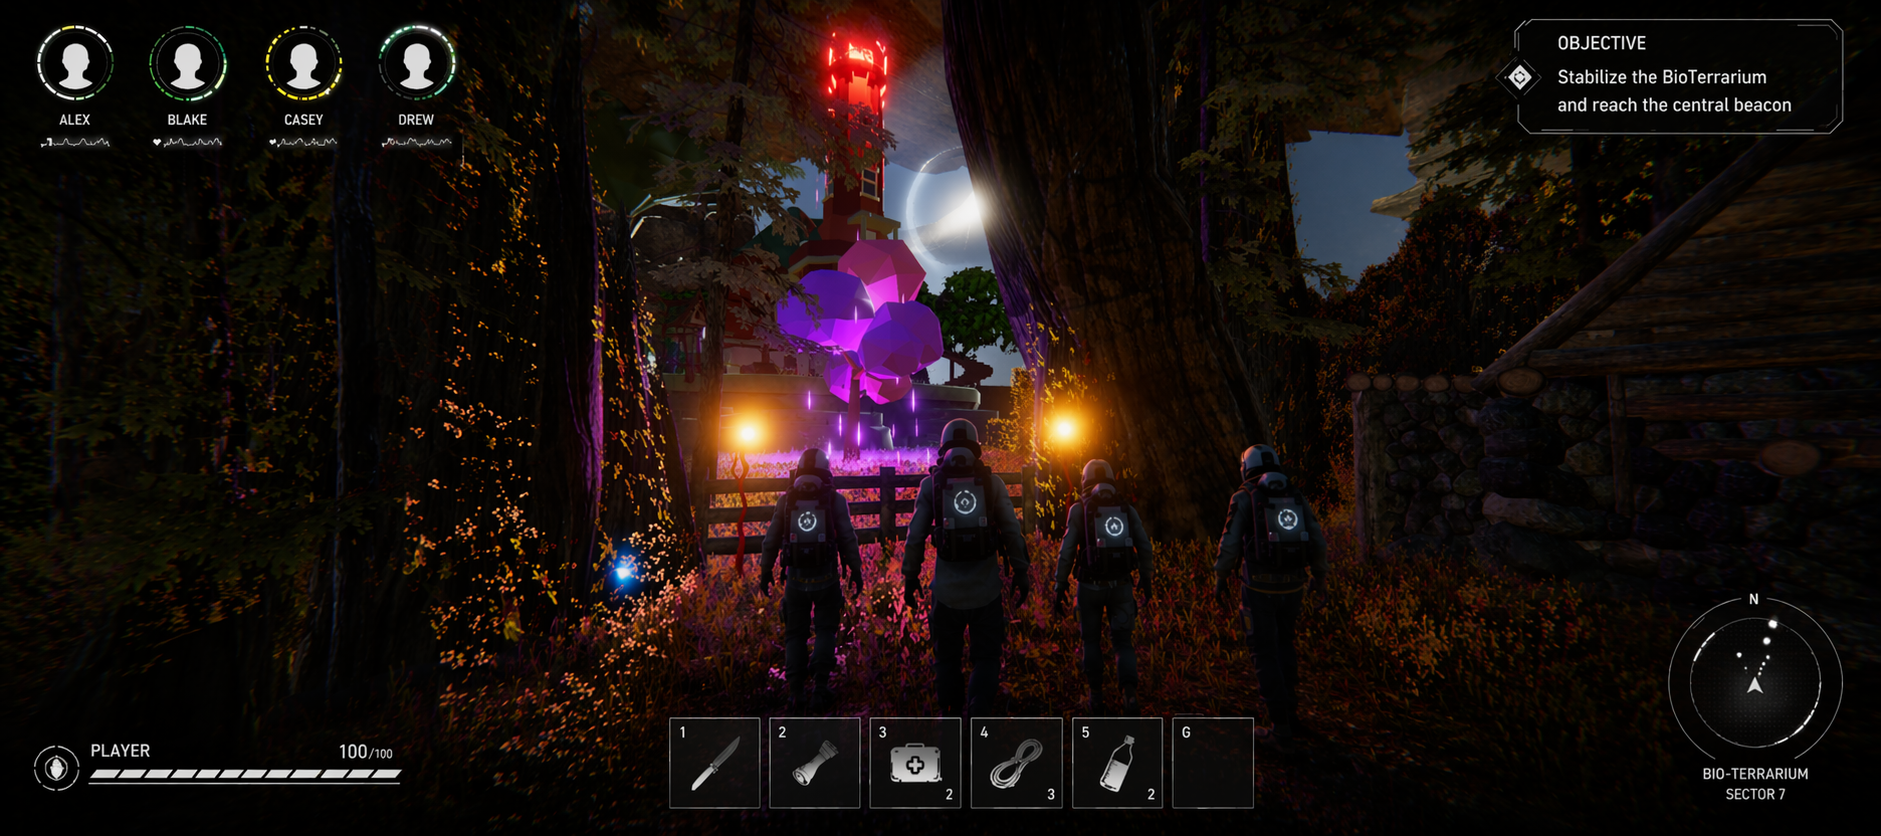
\includegraphics[width=\textwidth]{new interface.png}
  \caption{The BioTerrarium prototype visualizes players’ physiological signals through dynamic halos around avatar icons. HR and HRV are communicated as ambient visual cues supporting coordination during cooperative play.}
  \Description{A multiplayer game interface with player avatar icons surrounded by dynamic visual halos. The halos vary in pulse, density, brightness, and stability to communicate heart rate and heart-rate variability as ambient coordination cues.}
  \label{fig:teaser}
\end{teaserfigure}

%% remove fake received dates
% \received{20 February 2007}
% \received[revised]{12 March 2009}
% \received[accepted]{5 June 2009}

%%
%% This command processes the author and affiliation and title
%% information and builds the first part of the formatted document.
\maketitle

\section{Introduction}
Networked multiplayer games have become one of the largest settings where people cooperate with others they cannot see. Inside a single match, strangers and friends assemble into teams, divide roles, and steer shared outcomes through fast rounds of coordination. What holds such teams together is communication, and its quality tracks how well they perform: analyses of large player populations show that the volume and structure of team communication separate strong clans from weak ones \cite{bisberg_communication_2025}, and even a channel as thin as a map ping measurably shifts the result of a competitive match \cite{leavitt_ping_2016}. Coordination in these spaces rests on a stream of small signals that tell each member what the others attend to and how hard they are working.

One signal that teammates in a shared room read without effort never survives the trip across the network. When people occupy the same space, they register a partner's quickened breath, restless posture, and rising tension continuously and prereflectively, and they fold that reading into how they speak and act \cite{suchman_plans_1987, dourish_where_2004}. Distributed play strips this bodily layer away. A remote partner is left inferring effort, composure, and withdrawal from text, voice, and avatar motion, which carry far less than shared physical presence does. Controlled comparison confirms the cost: when the cues available in face to face contact are removed, collaborators understand one another less well, and judge one another more harshly, than when a representation of the partner's bodily state is restored \cite{tan_role_2014}.

The consequence is a specific failure of interpretation rather than a general lack of information. A teammate who has gone quiet may be concentrating, overloaded, or withdrawing, and the three call for opposite responses. Absent any read on the body, players guess, and wrong guesses accumulate into misattributed blame, mistimed help, and coordination that unravels under pressure. The problem this paper addresses is how to return a usable trace of that missing bodily layer to distributed teammates.

Sending physiological data across a network is not new. Heart rate has been carried into chat to raise empathy and awareness \cite{hassib_heartchat_2017}, into shared displays to deepen social connection \cite{slovak_understanding_2012, moge_shared_2022}, and into cooperative and virtual games to strengthen the felt bond between players \cite{jarvela_augmented_2021, hirsch_my_2023, jiang_intimasea_2023, muller_intra-_2013}. Two limits recur. First, a long affective computing tradition treats a biosignal as evidence for an underlying emotion to be detected and named \cite{picard_affective_1997, mandryk_fuzzy_2007}, fixing a single interpretation onto a body whose signals are notoriously ambiguous. Second, studies that report warmer feelings between partners seldom test whether a viewer can actually read the state on display and decide what to do about it, or whether the representation communicates anything once its emotion labels are removed. Legibility, and the situated judgment that follows from it, stays largely unmeasured.

We take a different route, and its shape comes from Science and Technology Studies. If measurement helps constitute the phenomenon it appears merely to record \cite{nelson_meeting_1996}, if the categories an interface imposes carry consequences of their own \cite{bowker_sorting_2008, winner_artifacts_1980}, and if every reading of a body belongs to a particular viewer and moment \cite{haraway_situated_1988}, then an interface that stamps a teammate's heartbeat with the word calm or panic overreaches. Our display withholds such verdicts. It renders Apple Watch heart rate as pulse rate and brightness, standing for cardiovascular activation, and heart rate variability as the coherence and steadiness of a ring, standing for autonomic regulation \cite{thayer_model_2000, porges_polyvagal_2007}. These become graded, deliberately open cues that a teammate weighs against the unfolding match rather than reads off as fact \cite{suchman_plans_1987, wakkary_things_2021}. The artifact is built to make an argument, not a diagnosis.

We evaluated whether that argument is even readable. In an online study, 36 distributed participants viewed all sixteen combinations of four heart rate states and four variability states and reported what each conveyed, through established instruments for symbol comprehension, affective rating, and workload. Participants recovered heart rate at 84 percent and variability at 81 percent from animation alone, well past the 25 percent expected from guessing. Their interpretations were ordered as the design intended: perceived urgency and arousal rose with activation, while falling variability coherence lowered perceived stability and raised the intention to offer support, none of it routed through emotion words. Reading the display cost little effort, most participants would accept it in cooperative play, and several drew boundaries around exposing bodily data to teammates, a concern we take up directly.

This paper contributes:
\begin{itemize}
\item a peripheral avatar display that turns wrist worn heart rate and variability into an ambient layer for reading a distant teammate, designed for the shared interactive space of a multiplayer match;
\item a design method that translates Science and Technology Studies commitments about measurement, classification, and situated knowledge into concrete visual choices, producing a representation that offers social cues without assigning emotions;
\item empirical evidence that this label free representation is legible, interpreted in a graded and consistent way, and light enough in workload to be usable, together with the privacy limits players place around it.
\end{itemize}

\section{Literature Review}

\subsection{Communication and Coordination in Distributed Play}
Multiplayer games reward study less as game systems than as places where scattered groups organize themselves. Communication volume and structure separate skilled teams from weak ones across large player populations \cite{bisberg_communication_2025}, and a signal as spare as a positional ping alters who wins a competitive round \cite{leavitt_ping_2016}. The channels behind these findings are deliberate and symbolic: messages, calls, pings. The involuntary bodily signals that regulate teamwork in a shared room, the ones a partner registers before either speaks \cite{suchman_plans_1987, dourish_where_2004}, reach the game through no channel at all. This section traces how prior work has tried to carry the body across a network, and where each attempt stops short of the reading a teammate needs.

\subsection{Reading Physiology as Emotion}
One tradition treats the body as a store of emotion to be recovered by computation. Affective computing set the agenda of sensing a signal and inferring the feeling behind it \cite{picard_affective_1997}, and play research applied it directly, mapping cardiac, muscular, and electrodermal activity onto models of a player's emotional state \cite{mandryk_fuzzy_2007, ravaja_phasic_2006} and adjusting game difficulty from those readings \cite{nacke_biofeedback_2011}. Surveys record both the reach of this approach and its persistent snag \cite{gan_human-computer_2022}: one elevated heart rate accompanies fear, exertion, and delight alike, so a system that prints a single emotion word onto it throws away the ambiguity the body genuinely carries. That interpretive move is the one our design declines.

\subsection{Sharing Physiology Between People}
A second line sends the signal to another person rather than to a classifier. Heart rate has been shared to build social connection \cite{slovak_understanding_2012, moge_shared_2022}, folded into mobile chat to lift empathy and awareness \cite{hassib_heartchat_2017}, and visualized during remote collaboration, where it raised group cohesion and perceived warmth over voice alone \cite{tan_role_2014}. In play, coupled and visualized biosignals have deepened the bond between partners in cooperative and virtual settings \cite{jarvela_augmented_2021, hirsch_my_2023, jiang_intimasea_2023, muller_intra-_2013}, consistent with evidence that physiological alignment tracks social closeness \cite{dikker_brain--brain_2017}. This work shows convincingly that a shared bodily signal changes how people relate. It leaves two things untested. It seldom asks whether a viewer can name the state on show, as distinct from feeling closer to its owner, and it seldom removes the emotional framing to check that the representation still communicates. Legibility, the precondition for acting on a cue mid match, is rarely the outcome measured.

\subsection{Situated Interpretation and a Science and Technology Studies Stance}
Where the first tradition locates meaning in the signal and the second in the bond, a third locates it in the moment of use. Situated and embodied accounts hold that action is read against an unfolding context rather than decoded from a fixed symbol \cite{suchman_plans_1987, dourish_where_2004}, and design research treats an artifact as a way to pose that question rather than close it \cite{wakkary_things_2021}. Science and Technology Studies sharpens the stakes for anything that measures a body: instruments help produce the phenomena they seem only to record \cite{nelson_meeting_1996}, classifications carry consequences for those they sort \cite{bowker_sorting_2008, winner_artifacts_1980}, and no reading of a body is a view from nowhere \cite{haraway_situated_1988}. Together these commitments argue against an interface that resolves a teammate's heartbeat into a verdict, and for one that offers a graded, open cue to be interpreted in place.

\subsection{Positioning the Present Work}
Two differences define this work against that background. Where shared physiology systems almost always transmit heart rate by itself, we add heart rate variability as a separate visual dimension, because the two indices carry different information: rate reflects momentary activation, while variability reflects the autonomic regulation underneath it \cite{thayer_model_2000, porges_polyvagal_2007}. And where earlier displays are judged by the connection they produce, we judge ours by the reading it supports, testing whether a label free representation is legible before asking what it does socially. Table~\ref{tab:related} sets the contrast out in full.

\begin{table}[t]
\footnotesize
\caption{Systems that carry physiological data between people, and how the present work differs. \emph{Emotion labels} marks whether the display names a feeling (Named), shows a raw or connection oriented signal that implies one (Implicit), or names none (None). \emph{Reader legibility} marks whether the study tested that a viewer can identify the intended state from the display itself.}
\label{tab:related}
\begin{tabular}{@{}l p{2.4cm} p{3.2cm} p{1.3cm} p{1.6cm}@{}}
\toprule
Work & Signal and setting & Primary aim & Emotion labels & Reader legibility tested \\
\midrule
Picard \cite{picard_affective_1997} & Multiple signals, no shared display & Recognize and model affect by computation & Named & No \\
Mandryk and Atkins \cite{mandryk_fuzzy_2007} & Cardiac, muscular, electrodermal in play & Infer a player's emotion from physiology & Named & No \\
Slov\'ak et al. \cite{slovak_understanding_2012} & Heart rate, shared display & Support social connection & Implicit & No \\
Hassib et al. \cite{hassib_heartchat_2017} & Heart rate, mobile chat & Raise empathy and awareness & Implicit & No \\
Tan et al. \cite{tan_role_2014} & Physiological signals, remote collaboration & Restore awareness and cohesion at a distance & Implicit & Indirect \\
Moge et al. \cite{moge_shared_2022} & Heart rate, cooperative game & Enrich shared play & Implicit & No \\
Hirsch et al. \cite{hirsch_my_2023} & Heartbeat, avatar in a VR game & Increase social connectedness & Implicit & No \\
\textbf{This work} & Heart rate and variability, peripheral avatar cue in distributed play & Make a teammate's state readable as a coordination cue & None & Yes \\
\bottomrule
\end{tabular}
\end{table}
\section{Methodology}
\noindent
\subsection{Research Methodological Orientation}
The research technique used in this study is positioned within the intersections of science and technology studies, game studies, and human–computer interaction. Research creation approaches allow theoretical problems to be investigated through material and creative practice by positioning the design and production of artefacts as essential components of scholarly inquiry. Research creation frameworks view constructed things and systems as places where knowledge may be created and explored, as opposed to treating artefacts as secondary results of research.
According to \cite {amos_kyriaki_2015}, research creation is a methodological paradigm where scholarly analysis and artistic output work together as mutually constitutive forms of knowledge formation. According to this approach, the creation of artefacts allows academics to investigate theoretical issues via design, experimentation, and reflection procedures. Using this methodological approach, the current study explores the potential translation of physiological sensing technologies into multiplayer interface components that influence players' perceptions and interpretations of one another during cooperative gaming.
Scholarship in Science and Technology Studies, which highlights that technological systems contribute to the creation of knowledge rather than serving as impartial tools of observation, further informs this study approach. According to \cite {nelson_meeting_1996}, measurement tools do more than just expose pre-existing characteristics of the world; they also contribute to the constitution of the phenomena they measure. In a similar vein, \cite {bowker_sorting_2008} show how classification systems integrated into technology infrastructures arrange the ways in which information becomes relevant and useful in social contexts. According to these viewpoints, physiological sensing technologies should be viewed as socio-technical arrangements that influence how physiological data is perceived and comprehended during interaction, in addition to being measuring tools.
The development of a technical system for physiological data sensing is not the only goal of the study within this methodological framework. Rather, the study looks at how physiological signal capture, classification, and visualisation might reorganise the interpretative conditions of multiplayer gaming.
\subsection{Research Creation as Design Inquiry}
Design practice serves as an inquiry method in research production that allows theoretical ideas to be investigated through the construction of artefacts. As a result, the artefact functions not only as a technological prototype but also as a research tool that makes it possible to examine specific issues related to social interaction and technology mediation. 
This methodological approach is consistent with human-computer interaction design research traditions that use artefacts as experimental systems to investigate different technology configurations and interaction paradigms. These methods enable researchers to investigate how new technology might change how people communicate, coordinate, and perceive in interactive settings.
The artifact developed in this study is a multiplayer physiological interface that visualizes players' physiological conditions through transformations in avatar icons during gameplay. Rather than aiming to optimize emotional detection or gameplay performance, the artifact is designed to explore how physiological signals may function as socially interpretable cues within cooperative gameplay contexts. Through the development of this artifact, the research examines how physiological visibility may influence how players interpret the actions and conditions of their teammates.



\begin{figure*}[t]
  \centering
  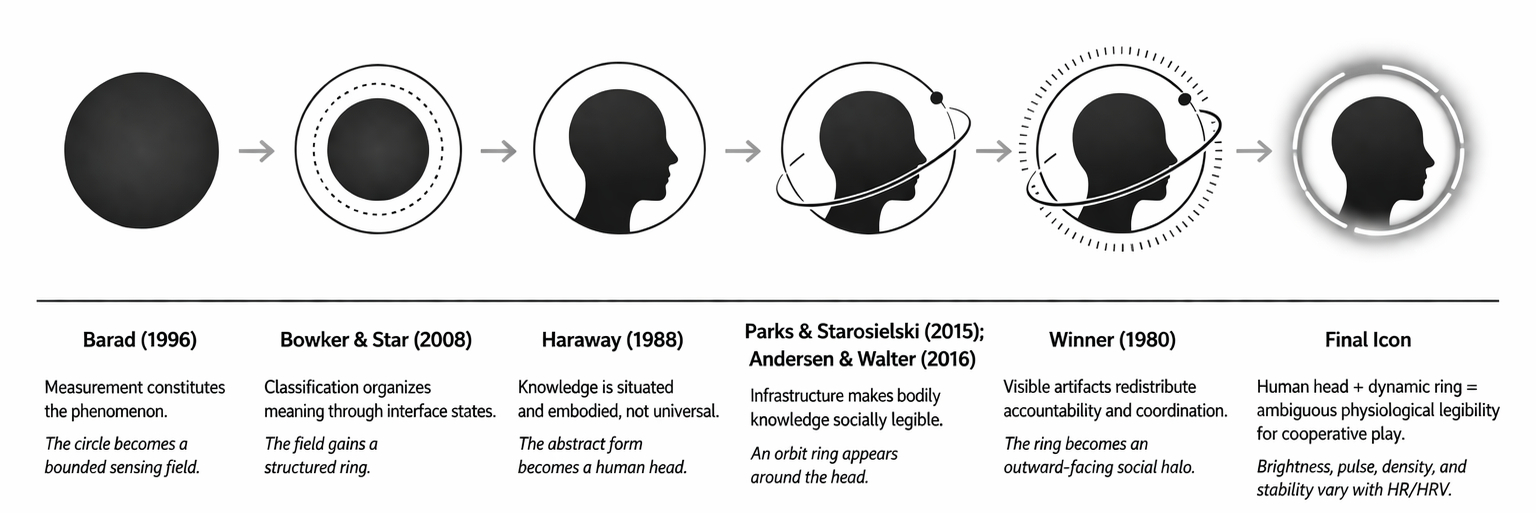
\includegraphics[width=\textwidth]{Icon.jpg}
  \caption{The icon design evolves through theoretical perspectives from Science and Technology Studies (STS), transforming an abstract sensing field into a human avatar surrounded by a dynamic halo. The final icon visualizes physiological signals as an ambiguous social cue, where halo brightness, pulse, density, and stability vary with heart rate (HR) and heart rate variability (HRV).}
  \Description{A visual design figure showing variations in avatar shapes and layered halo structures used to represent changes in heart rate and heart-rate variability.}
\end{figure*}

\subsection{Speculative Interface Design}
Speculative design methodologies, which employ conceptual artefacts to investigate alternative technology possibilities and challenge presumptions ingrained in current technological paradigms, also inform the project. According to \cite{wakkary_things_2021}, speculative design is a design approach that looks at how technologies might be structured differently from current technological trajectories. 
Artefacts serve as probes in speculative design, enabling researchers to investigate how specific technical configurations might change how people interact with technology systems. Speculative design makes it possible to investigate the wider conceptual and social ramifications of new technologies rather than concentrating just on their immediate practical uses.
The physiological interface proposed in this study therefore, functions as a speculative artifact that investigates how wearable biosensing technologies might become integrated into multiplayer game interfaces. Instead of assuming that physiological sensing should be used to infer emotional states or regulate gameplay performance, the design examines how physiological signals might operate as ambient and interpretable cues within collaborative play environments.
\subsection{Literature Driven Design Synthesis}
A synthesis of research from a number of pertinent fields, such as shared physiological interfaces, biofeedback game interaction, emotional computing, and Science and Technology Studies scholarship on measurement and categorisation, served as the basis for the conceptual creation of the artefact.
Affective computing research has shown how parts of human emotional experience and cognitive engagement may be modelled using physiological signals like heart rate and heart rate variability\cite{picard_affective_1997}. The integration of these signals into gameplay systems to affect player experience and interaction dynamics has been investigated in subsequent work in physiological game interaction \cite{mandryk_fuzzy_2007,nacke_biofeedback_2011}. Further research on shared physiological interfaces has demonstrated that social awareness and interpersonal coordination can be impacted by the visibility of physiological signals between people \cite{slovak_understanding_2012}. 
Scholarship in Science and Technology Studies offers a critical viewpoint on these advancements by highlighting the social and historical context of measurement techniques and classification schemes. According to\cite{bowker_sorting_2008}, classification schemes included in technical infrastructures influence how data is arranged and understood in social situations. In a similar vein, \cite{haraway_situated_1988}highlights that knowledge is not universally objective but rather local and incomplete. The design process purposefully avoided using explicit emotional labelling in the interface by drawing on these viewpoints. Instead of using rigid computational categories, physiological signals are viewed as contextual cues whose interpretation develops via interaction.
\subsection{System Development Process}
The artefact was developed through an iterative design process that was informed by both design exploration and theoretical thought. Finding ways to integrate physiological sensing technology into multiplayer interfaces without reducing physiological signals to explicit emotional classifications was the main goal of the early stages of development. In order to understand how physiological information may be portrayed in ways that maintain ambiguity while still enabling players to recognise changes in teammates' physiological status, alternative interface concepts were investigated.
The integration of wearable physiological sensors into the multiplayer interface concept was the main emphasis of later stages of development. The system architecture was created to integrate physiological data from wearable technology into the game's visual interface. A visual language that allows physiological variation to be conveyed through changes in player avatar icon appearance was created through iterative refinement. 
Decisions made throughout the design phase were assessed in light of the project's primary research goal, which is to investigate how physiological sensing technologies might alter the interpretive dynamics of cooperative gaming.
Early exploratory sketches were produced to investigate alternative visual strategies for embedding physiological signals into player avatar icons. These sketches explored variations in ring structure, pulsing behaviour, and inner avatar representation before the final halo-based visualization was established Figure 3.
\begin{figure*}[t]
  \centering
  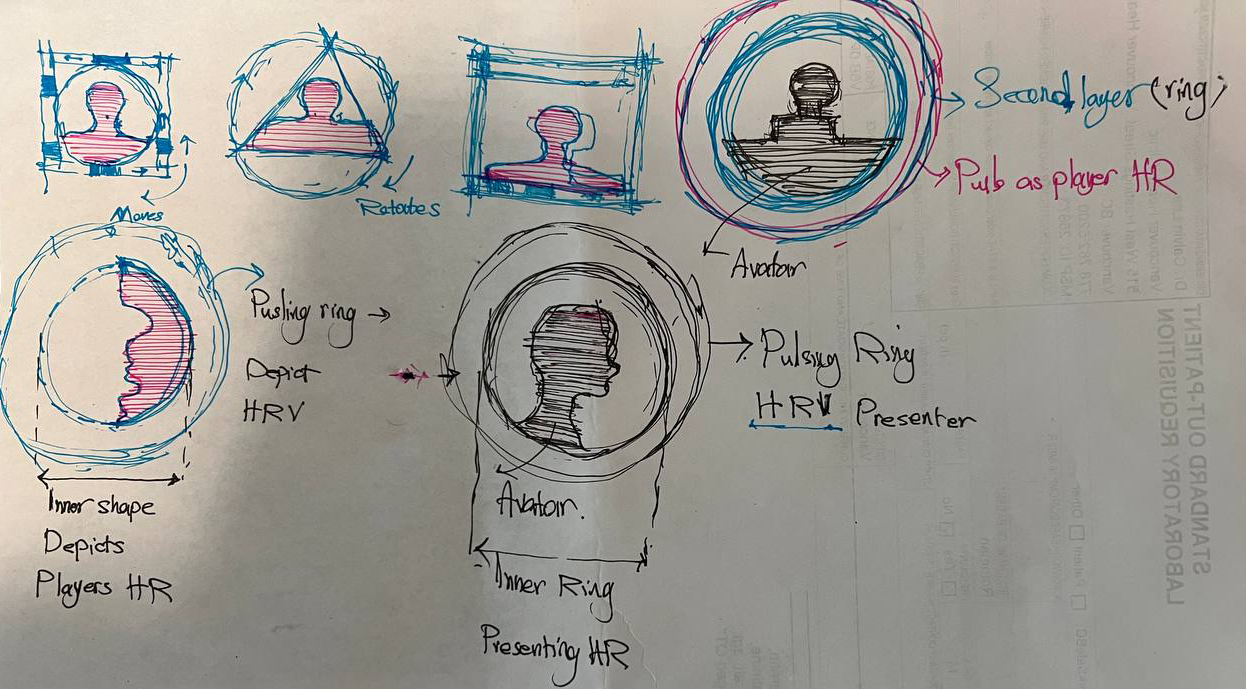
\includegraphics[width=\textwidth]{designprocess.png}
  \caption{Early design sketches exploring the visual representation of physiological signals in the avatar icon interface. The sketches investigate multiple configurations for embedding heart rate (HR) and heart rate variability (HRV) into the avatar visualization, including inner shape deformation, pulsating rings, and layered halo structures.}
  \Description{A visual design figure showing variations in avatar shapes and layered halo structures used to represent changes in heart rate and heart-rate variability.}
\end{figure*}
\subsection{Analytical Framework}
This study's analytical approach is based on human–computer interaction research theories of situated interaction and embodied involvement.\cite{suchman_plans_1987}contends that contextual interaction, as opposed to carrying out preconceived goals, is how human activity develops. In a similar vein,\cite{dourish_where_2004}highlights how embodied interaction with technology settings creates meaning in interactive systems. 
According to this viewpoint, whether or not physiological signals accurately reflect interior emotional states is not the main reason why physiological visualisation is important. Rather, its importance is seen in the way that physiological cues are integrated into the continuous processes of player interaction, coordination, and interpretation.
Therefore, the physiological interface created in this study can be used as an artefact to study the social effects of physiological visibility. Through the incorporation of physiological signals into multiplayer gaming, the system establishes novel circumstances for players to understand each other and negotiate cooperative behaviour.
\section{System Design}
\subsection{System Overview}
A multiplayer interface system that displays physiological signs from wearable devices during cooperative gaming is the artefact created in this study. By converting physiological measurements into visual cues that are incorporated into player avatar icons, the system enables players to notice changes in their colleagues' physiological states while engaging in gameplay. 
There are three main parts to the system architecture. The first part is the collection of physiological data using wearable sensors. A data processing layer that converts physiological measures into interface states makes up the second part. The third element is a visual interface layer that modifies the appearance of player avatar icons in the multiplayer interface to depict these statuses.
The technology communicates physiological variation through subtle visual modifications instead of using numerical displays or textual indications to present physiological information. Research indicates that ambient types of information visualisation can convey complicated data while maintaining the interpretative flexibility of the information being displayed, which is reflected in this design choice \cite{dourish_where_2004}.
\subsection{Physiological Data Acquisition}
Physiological data gathered from wearable technology, particularly the Apple Watch, is integrated into the system. The photoplethysmography sensors in the Apple Watch allow for continuous cardiovascular activity monitoring by detecting changes in blood volume beneath the skin. Applications can access physiological parameters, like as heart rate and heart rate variability, through the HealthKit framework.
Heart rate is a measure of transient cardiovascular stimulation and is expressed as the number of heartbeats per minute. Heart rate variability, which is commonly employed as a measure of autonomic nervous system function, represents fluctuation in the intervals between subsequent heartbeats. HRV can reveal information about cognitive load, stress, and emotional arousal during interactive tasks, according to physiological computing research \cite{mandryk_fuzzy_2007}.
In the proposed system, HR and HRV measurements are periodically retrieved from each player's wearable device and transmitted to the game environment. These measurements provide the physiological data upon which the interface visualization is based.
\subsection{Physiological Signal Interpretation}
The interface does not directly display raw physiological measurements. Rather, the system generates interface states that can be understood in the context of games by processing physiological data. 
Rather than trying to deduce particular emotional states, the interpretation layer concentrates on relative changes in physiological measures. The idea that physiological data may be directly mapped to distinct emotional categories has been criticised in both physiological computing and Science and Technology Studies \cite{haraway_situated_1988,bowker_sorting_2008}. As a result, the system uses patterns of cardiovascular activation obtained from heart rate and heart rate variability to interpret physiological inputs. The present physiological interface state is determined by taking into account both fluctuations in HRV and changes in heart rate relative to previous baseline values.
 This process produces a simplified representation of physiological dynamics suitable for visual communication within multiplayer interaction.
\subsection{Avatar Icon Visualization}
A dynamic icon system integrated into the multiplayer user interface is used to visualise physiological conditions. An avatar symbol appears in the gaming interface to represent each participant. Each icon is surrounded by a visual halo whose appearance varies in reaction to physiological cues. 
By altering visual characteristics, including colour intensity, pulse rhythm, and structural stability, the visual halo functions as an ambient visualisation layer that conveys physiological diversity. The avatar's halo appears steady and gently lit when physiological parameters are largely stable. The halo may exhibit more noticeable pulsing or visual intensity as physiological stimulation rises. Sharper visual transitions or variations in the halo structure could result from more significant physiological variance.
This approach avoids explicit numerical indicators or textual labels. Instead, the interface provides players with visual cues that must be interpreted in relation to ongoing gameplay events and interactions with teammates.
\subsection{Interface Integration in Multiplayer Gameplay}
The multiplayer game interface has a physiological icon system that allows players to monitor their teammates' physiological status while working together on cooperative activities. Throughout games, teammates' icons appear in the user interface, enabling players to sense physiological indicators in addition to other gameplay information. 
The design is meant to facilitate situations where players have to interpret their teammates' behaviours and circumstances in the face of uncertainty. Players frequently have to ascertain whether a partner is having trouble, hesitating, or becoming more engaged during challenging cooperative gameplay situations. These judgements may be influenced by the additional layer of information introduced by the physiological icon system.
Importantly, the system does not attempt to communicate definitive emotional states. Instead, physiological cues function as contextual signals that players may incorporate into their ongoing interpretations of team dynamics and gameplay events.
\subsection{Design Rationale}
The theoretical viewpoint that physiological signals shouldn't be regarded as objective depictions of internal emotional states is reflected in the physiological interface's architecture. Rather, physiological signals are viewed as contextual cues whose significance is revealed through interaction. 
Technology systems actively influence how information takes on meaning in social situations, according to research in Science and Technology Studies\cite{nelson_meeting_1996,bowker_sorting_2008}. According to this viewpoint, physiological data visualisation in multiplayer interfaces is a type of infrastructural mediation that affects how players see one another while playing.
The icon-based visualization, therefore, intentionally preserves ambiguity while still enabling players to perceive physiological variation. By avoiding explicit emotional labels and numerical representations, the interface encourages players to interpret physiological signals in relation to the unfolding dynamics of cooperative play.
\section{Results and Design Outcomes}
\subsection{Overview of the Artifact}
The outcome of the research process is a speculative multiplayer interface system that integrates wearable physiological sensing into the visual language of cooperative gameplay. The artifact translates physiological signals obtained from wearable devices into visual cues embedded within player avatar icons. Through this interface, physiological measurements become perceptible to teammates during gameplay without being presented as numerical indicators or explicit emotional classifications.
The system connects wearable physiological sensing with multiplayer interaction through a layered architecture consisting of physiological data acquisition, signal interpretation, and visual interface representation. Physiological signals collected from wearable devices are processed and translated into visual transformations that appear in the multiplayer interface. These transformations are applied to avatar icons representing individual players, enabling participants to observe physiological variation as part of the shared gameplay environment.
The artifact, therefore, demonstrates how physiological sensing technologies can be incorporated into multiplayer game interfaces in ways that emphasize interpretive cues rather than explicit diagnostic feedback.
\subsection{Physiological Interface States}
Variations in cardiovascular readings from wearable devices are used by the artefact to generate a variety of interface states. The relative variations in heart rate and heart rate variability recorded during games serve as the basis for these states. The approach uses visual states that match patterns of cardiovascular activation to convey physiological variation rather than classifying physiological signals into emotional categories. 
The avatar icon is encircled by a constant halo that preserves its structural form and brightness under physiologically stable settings. There is very little change in heart rate and heart rate variability in this visual condition.
When cardiovascular activation increases relative to baseline measurements, the halo surrounding the icon begins to display rhythmic pulsing. This pulsing effect visually indicates changes in physiological activity while preserving the ambiguity of the underlying signal.
Increased visual alterations in the halo structure are caused by more noticeable physiological fluctuation. Under these circumstances, the halo may exhibit rapid pulsation patterns or increased luminosity, which enhance the physiological signal's visibility within the interface. 
The halo may exhibit unstable visual properties, such as irregular pulsing or visual distortion, when physiological signals show significant variations. While avoiding the presentation of overtly emotional interpretations, these changes convey important physiological variance.
\subsection{Avatar Icon Visualization}
Within the multiplayer interface, each player's avatar icon incorporates a visual halo that represents physiological data. The halo serves as an ambient visualisation layer that uses changes in visual characteristics, such as brightness, rhythm, and structural stability, to convey physiological changes. 
This visualisation technique does not use textual indications or numerical values. Rather, the interface uses dynamic visual components that are integrated into the multiplayer interface's current visual framework to convey physiological indications. 
Physiological signals become a part of the visual environment via which players perceive their colleagues' state because the halo is visible during games.
Changes in the halo are continuously updated in response to incoming physiological measurements, allowing the interface to reflect ongoing physiological variation.

\subsection{Integration Within Multiplayer Gameplay}
Alongside other gameplay interface components, teammates' avatar icons can be seen within the game area. As physiological measures are updated, each icon's surrounding physiological halo dynamically changes. Players can concurrently focus on gameplay goals and surrounding events while simultaneously perceiving physiological cues thanks to this design. 
In order to avoid taking over the visual interface, the physiological visualisation is purposefully unobtrusive. Rather, the halo functions as a peripheral indicator that players may observe and decipher when pertinent to the current gameplay scenario. 
The artefact adds physiological sensing as an extra layer of information in cooperative gaming through this design. As a result, during cooperative activities, players use physiological cues as part of the interpretative environment to coordinate actions and decipher colleagues' behaviour.
\subsection{Artifact Outcome}
The main result of the research process is the creation of a conceptual physiological interface that shows how ambient visualisation techniques can be used to include wearable cardiovascular sensors into multiplayer game interfaces. Without explicitly showing physiological measures as emotional classifications, the artefact demonstrates how physiological data might be converted into visual signals that help players' interpretive awareness. 
The interface incorporates physiological sensing into the visual language of online gaming by including physiological visualisation into avatar icons. This design result lays the groundwork for investigating how player interpretation, cooperation, and engagement in cooperative digital environments may be impacted by physiological visibility.
\section{Discussion}
\subsection{Physiological Visibility in Multiplayer Interaction}
By converting cardiovascular signals into visual changes incorporated into player avatar icons, the artefact created in this study adds a type of physiological visibility to online gaming. During cooperative contact, teammates can perceive physiological parameters via wearable sensing devices thanks to this interface. The interface conveys physiological fluctuation using ambient visual cues incorporated into the gaming world, as opposed to displaying physiological data as numerical indicators or explicit emotional labelling. 
Players frequently use incomplete and context-dependent information to interpret their colleagues' intents and actions during cooperative games. Players can deduce the circumstances and intentions of others by using communication channels like movement, time, and environmental interaction. In this interpretive environment, the physiological interface adds another layer of information.
The technology offers cues that could affect how players perceive reluctance, risk-taking, or participation during cooperative gameplay by making physiological variation visible through avatar icons. 
From the standpoint of embodied interaction, these cues are more significant in how they are integrated into ongoing engagement than in how accurately they represent internal emotional states. Instead of merely transmitting symbolic representations, meaning in interactive systems arises through situated involvement with technical surroundings \cite{dourish_where_2004}. According to this theory, players use the physiological visualisation as a contextual signal for interpreting what is happening in the game.
\subsection{Measurement and the Mediation of Physiological Signals}
The system also demonstrates how technology infrastructures have a mediation role in determining how physiological signals are interpreted in digital contexts. The interface does not receive physiological signals obtained via wearable technology as unprocessed biological data. Rather, they go through a series of sensing, processing, categorisation, and visualisation processes that decide how those signals appear in the interface. 
Scholarship in Science and Technology Studies has highlighted how measurement tools contribute to the creation of the phenomena they seem to witness.
Barad contends that rather than only disclosing preexisting characteristics of the environment, measurement tools actively contribute to the composition of the phenomena they measure \cite{nelson_meeting_1996}. Wearable sensors, data processing algorithms, and visual interface components work together to create the physiological interface created in this study, which makes cardiovascular activity visible in a multiplayer setting. 
Therefore, it is not appropriate to interpret physiological signals provided by avatar symbols in this configuration as clear indicators of players' interior states. Rather, they serve as mediated signals whose meaning develops via the interplay of player interpretation, interface design, and sensing technology.
\subsection{Classification and Interface Representation}
Classifying physiological signals is a major design problem in physiological interface systems. Physiological signals are often mapped onto distinct emotional categories like stress, enthusiasm, or frustration by physiological computing systems. These methods frequently make the assumption that certain emotional states may be accurately correlated with physiological measures. 
The interface created for this study purposefully steers clear of overt emotional classification. Rather, physiological inputs are converted into visual interface states that convey changes in cardiovascular activity without imposing predetermined emotional interpretations. Critical viewpoints on classification schemes created within Science and Technology Studies are reflected in this design choice.
\cite{bowker_sorting_2008} demonstrates that classification systems embedded within technological infrastructures shape how information becomes organized and interpreted within social contexts\cite{bowker_sorting_2008}. Once implemented, classification categories can become naturalized as objective representations of the phenomena they describe. In the context of physiological sensing, rigid emotional classifications risk presenting physiological measurements as definitive indicators of subjective experience.
By representing physiological variation through ambiguous visual transformations rather than explicit emotional labels, the interface allows the meaning of physiological signals to emerge through interaction with gameplay context.
\subsection{Situated Interpretation of Physiological Data}
The idea of contextual knowledge can also be used to comprehend the interpretive nature of physiological visualisation. According to \cite{haraway_situated_1988}, knowledge claims are never generated from universal or disembodied views, but rather from particular positions and situations \cite{haraway_situated_1988}. Similar to this, physiological signals are incorporated in the specific conditions of measurement and interpretation. 
Similar physiological characteristics may be associated with different experiencing situations in gaming contexts. Depending on the actual context of play, increased cardiovascular activation may indicate focus, excitement, cognitive exertion, or uncertainty. This ambiguity is not addressed by the physiological interface created in this study. Rather, it sends signals that players have to decipher in light of current gameplay events and team relations.
This approach acknowledges the contextual nature of physiological information and avoids presenting physiological sensing technologies as capable of producing definitive interpretations of internal experience.
\subsection{Technological Visibility and Multiplayer Coordination}
The way that technology systems influence player engagement is also affected by the incorporation of physiological sensors into multiplayer interfaces. By influencing how information is made accessible to participants, technological artefacts can affect patterns of perception, coordination, and accountability within social systems. 
 \cite{winner_artifacts_1980} contends that by organising the distribution of information and actions inside technological systems, technical artefacts may represent certain configurations of power and authority. The choice to make physiological signals visible to teammates modifies the cooperative game's informative landscape in the interface suggested in this study. 
During cooperative tasks, physiological visibility may affect how players assess risk, decipher hesitancy, or assign blame.
The interface, therefore, participates in shaping the interpretive dynamics of multiplayer interaction by introducing a new form of physiological legibility within the game environment.
\subsection{Implications for Physiological Game Interfaces}
An alternate method of incorporating physiological sensing into video games is suggested by the artefact created in this study. The utilisation of physiological signals to improve gameplay performance, adjust game difficulty, or deduce player emotions has been the main focus of much of the current physiological computing research. The interface suggested here emphasises the social and interpretive aspects of physiological visibility, whereas these methods focus on the computational interpretation of physiological data. 
The approach enables physiological data to serve as contextual signals in multiplayer interaction by using ambient visual cues to represent physiological signals instead of explicit emotional markers. By doing this, the interface changes the function of physiological sensing in cooperative gaming from an emotional detection mechanism to a medium of interpretive awareness.
\section{Limitations}
When analysing the suggested interface design, it is important to take into account the constraints that this study offers. The system is based on physiological signals that are collected from wearable sensors that detect heart rate and heart rate variability. These signals do not specifically correlate to particular emotional or cognitive states, even if they offer markers of circulatory activity. Numerous factors, such as stress, focus, or physical effort, can cause similar physiological responses. Cardiovascular signals by themselves are unable to definitively interpret subjective experience, according to research in physiological computing \cite{mandryk_fuzzy_2007}. Because of this, the interface depicts physiological variance through visual signals that are subject to interpretation within the context of gameplay rather than explicitly labelling emotions.
Another limitation concerns the speculative nature of the artifact. The system was developed through a research creation methodology as a conceptual design intended to explore how wearable physiological sensing might be integrated into multiplayer interfaces. The study, therefore, emphasizes conceptual development and theoretical implications rather than empirical evaluation through large-scale user testing. Further research would be necessary to examine how players interpret and respond to physiological visualization during extended gameplay sessions.
The system depends on physiological measurements obtained from wearable sensing devices such as the Apple Watch. Wearable photoplethysmography sensors are subject to limitations, including signal noise, motion artifacts, and sampling constraints that may affect measurement stability during gameplay. In addition, the visibility of physiological signals within multiplayer environments raises ethical and privacy considerations related to the sharing of personal biological data. Future implementations of physiological multiplayer interfaces would need to address issues of consent, data ownership, and control over the visibility of physiological information.
\section{Conclusion}
This work introduced a hypothetical multiplayer interface that visualises heart rate and heart rate variability inputs from wearable devices to incorporate physiological sensing into cooperative gaming. In order to enable teammates to notice physiological change during gameplay without depending on numerical displays or explicit emotional classification, the proposed system converts physiological measurements into ambient visual transformations integrated into player avatar icons. 
The study looked at how physiological sensing technologies might be used as interface components that influence interpretation and coordination in multiplayer interaction, in addition to serving as instruments for gauging participant states. The research investigated how processes of sensing, categorisation, and visualisation affect how physiological information becomes meaningful inside digital settings, drawing on viewpoints from human-computer interaction and Science and Technology Studies.
The interface highlights the interpretative and socially controlled character of physiological data by portraying physiological signals as contextual visual clues rather than conclusive markers of interior emotional states. As a result, the artefact illustrates a different strategy for incorporating physiological sensing into game interfaces, one that prioritises awareness, interpretation, and cooperative interaction above deterministic emotional detection. 
The study adds to existing debates on the use of biometric sensing technologies in interactive systems in the fields of human-computer interaction, game design, and Science and Technology Studies. The impact of physiological visualisation on player coordination, perception, and communication in cooperative digital settings may be further studied in the future.
\section{Generative AI Use Disclosure}
ChatGPT was used for language editing and restructuring text drafted by the author. It was not used to generate the research idea, conceptual framework, study design, data, results, or citations. The author reviewed and takes responsibility for all content.

% Identifying acknowledgments are omitted for blind review.
%%%%%%%%%%%%%%%%%%%%%%%%%%%%%%%%%

%%%%%%%%%%%%%%%%%%%%%%%%%%%%%%%%%%

%%%%%%%%%%%%%%%%%%%%%%%%%%%%%%%%%%%%%%


%%%%%%%%%%%%%%%%%%%%%%%%%%%%%%%%%%%
\FloatBarrier  % stops earlier figures
\clearpage     % flushes all previous floats

\bibliographystyle{ACM-Reference-Format}
\bibliography{sample-base}


\FloatBarrier  % stops earlier figures from floating here
\clearpage     % flushes all previous floats


\FloatBarrier  % stops earlier figures from floating here
\clearpage     % flushes all previous floats





%%%%%%%%%%%%%%%%%%%%%%%%%%%%%%%%%%%%%%%%%

\FloatBarrier  % stops earlier figures from floating here
\clearpage     % flushes all previous floats




% --- Figure 2 code ---



\FloatBarrier  % stops earlier figures from floating here
\clearpage     % flushes all previous floats




\end{document}
\endinput
%%
%% End of file `sample-sigconf-authordraft.tex'.
